\documentclass[12pt]{scrartcl}

\usepackage{amsthm}
\usepackage{ocgx}
\usepackage{amsmath}
\usepackage{graphicx}

\title{Lecture Notes week 1}
\author{\"Omer \c Sakar}
\date{\today}

\newtheorem{defi}{Definition}
\newtheorem{theo}{Theorem}

\usepackage{tikz}
\usetikzlibrary{shapes,backgrounds}


\begin{document}
\maketitle
\tableofcontents
\newpage

\section{Lecture 1}

\subsection{Bayes' Rule}
Given events $A$ and $B$:\newline

\begin{defi}
 	The Conditional Probability $P(A | B) = \frac{P(A \cap B) }{P(B)},\ 	 with\ P(B)\ >\ 0.$
\end{defi}

\begin{figure}[h]
	\centering
	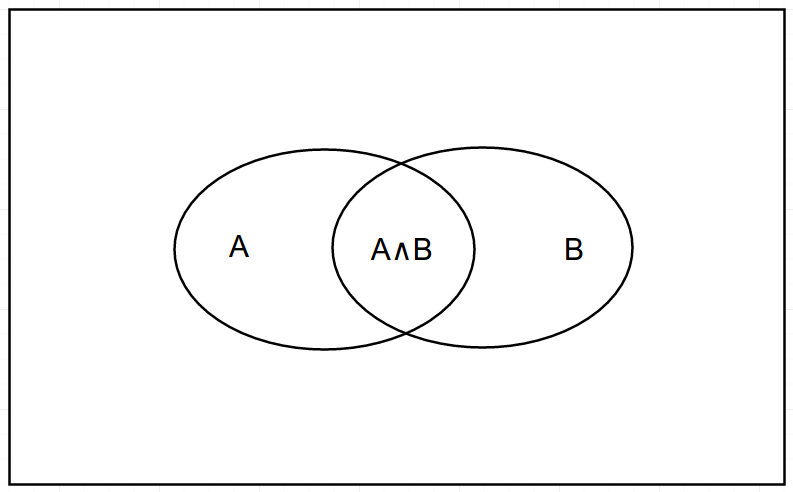
\includegraphics[width=0.3\textwidth]{./images/venn_diagram.png}
	\captionof{figure}{Visual representation of Bayes' Rule}    
    \label{fig:formal_proof_ties}
\end{figure}

Example: There are 40 Math students of which 15 are girls and there are 50 Computer Science students of which 10 are girls.\newline
Let $A\ =\ randomly\ chosen\ student\ is\ a\ girl$ and $B\ =\ randomly\ chosen\ student\ is\ a\ math\ student$.
\newline

$P(A | B) = \frac{P(A \cap B)}{P(B)} = \frac{\ \ \frac{15}{90}\ \ }{\frac{40}{90}} = \frac{3}{8}$\newline

\noindent And from Bayes' Rule follows $\Rightarrow P(A \cap B) = P(A | B)\cdot P(B) = P(B|A)\cdot P(A), P(A) > 0$.

Thus we can rewrite it as:
\begin{defi}
 	The Conditional Probability $P(B | A) = \frac{P(A | B)\cdot P(B) }{P(A)}.$
\end{defi}

\subsubsection{Full Probability Formula}
\begin{defi}
	$P(A) = P(B) \cdot P(A | B) + P(\bar{B})\cdot P(A | \bar{B})$
\end{defi}
\noindent Example: $P(B | A) = \frac{P(A | B)\cdot P(B)}{P(A)} = \frac{\ \frac{40}{90}\cdot \frac{3}{8}\ }{\frac{25}{90}} = \frac{3}{8}$\newline

\subsection{A Herding Experiment}
Envelope 1 contains 8 red and 4 blue domino pieces (R) and envelope 1 contains 4 red and 8 blue domino pieces (B).\newline
$P(R) = P(B) = \frac{1}{2} $\newline
The first person that draws either a red or blue piece.\newline
$P(R | (saw) blue) = \frac{P(blue | R)\cdot P(R)}{P(blue)}$.

\noindent$P(blue) = P(R)\cdot P(blue |R) + P(B)\cdot P(blue | B) = \frac{1}{2}\cdot \frac{4}{12} + \frac{1}{2}\cdot \frac{8}{12} = \frac{1}{2}$

\noindent$P(R | blue) = \frac{\frac{4}{12}\cdot \frac{1}{2}}{\frac{1}{2}} = \frac{1}{3} < \frac{1}{2}\
 and\ P(B | blue) = \frac{\frac{8}{12}\cdot \frac{1}{2}}{\frac{1}{2}} = \frac{2}{3} > \frac{1}{2}$



\noindent Now lets look at when a second person draws.
\begin{defi}
	$D_{i} = \{blue\}\ or\ \{red\}\ -\ what\ person\ i\ says\ they\ saw$
\end{defi}
\begin{defi}
$E_{i} = \{blue\}\ or\ \{red\}\ -\ what\ person\ i\ saw$
\end{defi}
\noindent Lets say that the first person says what he sees ($D_{1} = E_{1}$)

\noindent$P(B | blue, blue) = \frac{P(B)\cdot P(blue, blue | B)}{P(blue, blue)}$

\noindent$P(blue, blue) = \frac{1}{2}\cdot (\frac{2}{3})^{2} + \frac{1}{2}\cdot (\frac{2}{3})^{2} = \frac{5}{18}$

\noindent Thus $P(B | blue, blue) = \frac{\frac{1}{2}\cdot (\frac{2}{3})^{2}}{\frac{5}{18}} = \frac{4}{5} > \frac{1}{2}$

\noindent Conclusion: If $D_{1} = \{blue\}$ and $E_{2} = \{blue\} \implies D_{2} = \{blue \}$\newline

\noindent $P(R) = P(B) = \frac{1}{2}$\\
$P(B | blue, red) = \frac{P(B)\cdot P(blue, red | B)}{P(blue, red)} = \frac{\frac{1}{2}\cdot \frac{2}{3}\cdot \frac{1}{2}}{ \frac{1}{2}\cdot \frac{2}{3}\cdot \frac{1}{2} + \frac{1}{2}\cdot \frac{2}{3}\cdot \frac{1}{2}} = \frac{1}{2}$\\
$D_{1} = \{blue\}, E_{2} = \{red\} \implies D_{2} = \{red\}$
If your opinions differ then




\noindent$P(B cascade| R) = \frac{1}{3}\cdot \frac{1}{3} + (\frac{1}{3}\cdot \frac{2}{3})\cdot 2\cdot \frac{1}{3}\cdot \frac{1}{3} + 
(\frac{1}{3}\cdot \frac{2}{3}\cdot 2)^{2}\cdot \frac{1}{3}\cdot \frac{1}{3} + \cdots
= \frac{1}{9}\cdot \frac{1}{1 - \frac{4}{9}} = \frac{1}{5} \equiv 20\%$
\subsection{Genral Cascade Model}
Example: Adopting a product\newline
1) Let B be bad and G be good. We estimate $P(B) = 1-p$ and $P(G) = p$.\newline
2) And let $v_{g}$ be if we guess G right and $v_{b}$ if we guess B right.\newline
$v_{g}\cdot p + v_{b}\cdot (1-p) = 0$ - Expected Reward. Rewritten it looks like $v_{b} + (v_{g} - v_{b})\cdot p$.\newline
It is accepted if $P(G|signal) > p$ and rejected if $P(G | signal) < p$.

\noindent 3) low(L) and high(H)
\begin{table}[h]
\centering
\begin{tabular}{|l|l|l|}
\hline
  & B   & G   \\\hline
L & q   & 1-q \\\hline
H & 1-q & q  \\\hline
\end{tabular}
\caption{With q $> \frac{1}{2}$}
\label{my-label}
\end{table}

\noindent $P(L|B) = q > \frac{1}{2},\ P(H|B) = 1-q$. $P(L|G) = 1-q,\ P(H|G) = q > \frac{1}{2}$.\newline

\noindent First person $P(G|H) = \frac{P(H|G)\cdot P(G)}{P(H)} = \frac{p\cdot q}{p\cdot q + (1-p)\cdot (1-q)} > \frac{p\cdot q}{p\cdot q + (1-p)\cdot q} = \frac{p\cdot q}{q} = p$\newline
Thus $E_{1} = \{H\}\implies D_{1} = \{G\}$\newline

\noindent Let $a+b$ - person and $S$ - signal a times H and b times L.

\noindent $P(G|S) = \frac{P(S|G)\cdot P(G)}{P(S)} = \frac{p\cdot q^{a}\cdot (1-q)^{b}}{p\cdot q^{a}\cdot (1-q)^{b} + (1-p)\cdot (1-q)^{a}\cdot q^{b}} > \frac{p\cdot q^{a}\cdot (1-q)^{b}}{p\cdot q^{a}\cdot (1-q)^{b} + (1-p)\cdot q^{a}\cdot (1-q)^{b}} = p$

\noindent This is when $a < b \iff (1-q)^{a}\cdot q^{b} > q^{a}\cdot (1-q)^{b}$ (because $q>1-q$). 

\noindent Thus when $a < b, D = \{B\}$

\noindent If $a > b \iff (1-q)^{a}\cdot q^{b} < q^{a}\cdot (1-q)^{b}$ . This would result in $P(G|S) > p \implies D = \{G\}$

//TODO insert picture of graph

\newpage
\section{Lecture 2} 


\end{document}




